% This file was converted to LaTeX by Writer2LaTeX ver. 1.0.2
% see http://writer2latex.sourceforge.net for more info
\documentclass[11pt]{article}
\usepackage[utf8]{inputenc}
\usepackage[T1]{fontenc}
\usepackage[english]{babel}
\usepackage{amsmath}
\usepackage{amssymb,amsfonts,textcomp}
\usepackage{array}
\usepackage{supertabular}
\usepackage{hhline}
\usepackage{hyperref}
\hypersetup{colorlinks=true, linkcolor=blue, citecolor=blue, filecolor=blue, urlcolor=blue}
\usepackage{graphicx}
% Text styles
\newcommand\textstyleListLabeli[1]{{\fontsize{16pt}{19.2pt}\selectfont \textrm{\textbf{\textup{#1}}}}}
\makeatletter
\newcommand\arraybslash{\let\\\@arraycr}
\makeatother
\raggedbottom
% Paragraph styles
\renewcommand\familydefault{\rmdefault}
\newenvironment{styleNormali}{\setlength\leftskip{0cm}\setlength\rightskip{0cm plus 1fil}\setlength\parindent{0cm}\setlength\parfillskip{0pt plus 1fil}\setlength\parskip{0cm plus 1pt}\writerlistparindent\writerlistleftskip\leavevmode\normalfont\normalsize\writerlistlabel\ignorespaces}{\unskip\vspace{0cm plus 1pt}\par}
% List styles
\newcommand\writerlistleftskip{}
\newcommand\writerlistparindent{}
\newcommand\writerlistlabel{}
\newcommand\writerlistremovelabel{\aftergroup\let\aftergroup\writerlistparindent\aftergroup\relax\aftergroup\let\aftergroup\writerlistlabel\aftergroup\relax}
\newcounter{listWWNumiileveli}
\newcounter{listWWNumiilevelii}[listWWNumiileveli]
\newcounter{listWWNumiileveliii}[listWWNumiilevelii]
\newcounter{listWWNumiileveliv}[listWWNumiileveliii]
\renewcommand\thelistWWNumiileveli{\arabic{listWWNumiileveli}}
\renewcommand\thelistWWNumiilevelii{\arabic{listWWNumiileveli}.\arabic{listWWNumiilevelii}}
\renewcommand\thelistWWNumiileveliii{\arabic{listWWNumiileveli}.\arabic{listWWNumiilevelii}.\arabic{listWWNumiileveliii}}
\renewcommand\thelistWWNumiileveliv{\arabic{listWWNumiileveli}.\arabic{listWWNumiilevelii}.\arabic{listWWNumiileveliii}.\arabic{listWWNumiileveliv}}
\newcommand\labellistWWNumiileveli{\thelistWWNumiileveli.}
\newcommand\labellistWWNumiilevelii{\textstyleListLabeli{\thelistWWNumiilevelii.}}
\newcommand\labellistWWNumiileveliii{\thelistWWNumiileveliii.}
\newcommand\labellistWWNumiileveliv{\thelistWWNumiileveliv.}
\newenvironment{listWWNumiileveli}{\def\writerlistleftskip{\addtolength\leftskip{0.0cm}}\def\writerlistparindent{}\def\writerlistlabel{}\def\item{\def\writerlistparindent{\setlength\parindent{-0cm}}\def\writerlistlabel{\stepcounter{listWWNumiileveli}\makebox[0cm][l]{\labellistWWNumiileveli}\hspace{0cm}\writerlistremovelabel}}}{}
\newenvironment{listWWNumiilevelii}{\def\writerlistleftskip{\addtolength\leftskip{0.0cm}}\def\writerlistparindent{}\def\writerlistlabel{}\def\item{\def\writerlistparindent{\setlength\parindent{-0cm}}\def\writerlistlabel{\stepcounter{listWWNumiilevelii}\makebox[0cm][l]{\labellistWWNumiilevelii}\hspace{0cm}\writerlistremovelabel}}}{}
\newenvironment{listWWNumiileveliii}{\def\writerlistleftskip{\addtolength\leftskip{0.0cm}}\def\writerlistparindent{}\def\writerlistlabel{}\def\item{\def\writerlistparindent{\setlength\parindent{-0cm}}\def\writerlistlabel{\stepcounter{listWWNumiileveliii}\makebox[0cm][r]{\labellistWWNumiileveliii}\hspace{0cm}\writerlistremovelabel}}}{}
\newenvironment{listWWNumiileveliv}{\def\writerlistleftskip{\addtolength\leftskip{0.0cm}}\def\writerlistparindent{}\def\writerlistlabel{}\def\item{\def\writerlistparindent{\setlength\parindent{-0cm}}\def\writerlistlabel{\stepcounter{listWWNumiileveliv}\makebox[0cm][l]{\labellistWWNumiileveliv}\hspace{0cm}\writerlistremovelabel}}}{}
\setlength\tabcolsep{1mm}
\renewcommand\arraystretch{1.3}
% footnotes configuration
\makeatletter
\renewcommand\thefootnote{\arabic{footnote}}
\makeatother
\title{}
\author{UIC}
\date{2018-01-19}
\begin{document}
\title{The second time around: the effect of formal instruction on VOT production upon return from study abroad}
\maketitle

\begin{styleNormali}
The present study aims at assessing~L2 phonological development,~while controlling for proficiency level, as a result of~a 2-month formal instruction (FI) period following a 3-month period spent abroad in a country where the learners’ target language was spoken. It examines voice onset time (VOT) production of English voiceless stops in initial stressed position by Catalan/Spanish EFL learners. It is intended as a follow-up of Mora{\textquotesingle}s (2008) study, which yielded no significant effects at the end of the stay abroad (SA) only. It is hypothesized that the FI period should allow students to focus on their phonology, away from the pressing demands of daily communication during SA. No explicit attention is paid to phonology in class. Speech samples were collected from 13 participants, through two tasks, upon their return from SA and immediately after a 2-month period of FI. No significant effect of the FI period preceded by a SA term on informants’ VOTs was found. Proficiency level seems to have played a role in VOT production. Speaking style, vowel height and place of articulation were found to significantly affect VOT production of voiceless stops, in line with previous findings. A baseline group of natives showed the same numerical tendency.~The lack of impact resulting from a FI period preceded by a SA term adds further support for the suggestion made by some authors (Darcy et al. 2012; Gordon \& Darcy 2012; Calvo Benzies 2014) that explicit attention to phonology in FI should act as a potential factor to effectively improve L2 phonological development.
\end{styleNormali}


\setcounter{listWWNumiileveli}{0}
\begin{listWWNumiileveli}
\item 
\begin{styleNormali}
\textbf{Introduction}
\end{styleNormali}

\end{listWWNumiileveli}
\begin{styleNormali}
It is often assumed that L2 oral speech development will improve as a result of stay abroad (SA), whereas less improvement will be noted as a consequence of formal instruction (FI). However, there is little evidence to support this claim, as studies assessing second language (L2) phonological acquisition resulting from a SA are still scarce and results are conflicting. Importantly, phonological development seems to be one of the most challenging aspects of L2 acquisition for learners, a fact that is likely due to a lack of a consistent pedagogical methodology in teaching (Darcy et al. 2012). 
\end{styleNormali}


\begin{styleNormali}
Hence, this empirical study aims at continuing to fill the existing research gap in L2 speech production. The study has been carried out within the Study Abroad and Language Acquisition (SALA) project (see Pérez-Vidal 2014), where linguistic and non-linguistic progress as a function of SA are analysed, including L2 phonological development. FI has also been examined in combination with SA within the project. However, FI periods preceded SA ones in the SALA studies. Our work seeks to provide a counterbalanced perspective by examining the impact of an FI period following a SA.
\end{styleNormali}


\begin{styleNormali}
In order to obtain as thorough an understanding of L2 phonological development as possible, the interplay of three important connected aspects is explored in the literature review: (i) the teaching of pronunciation in the classroom, (ii) the linguistic outcomes obtained as a function of learning context, and (iii) voice onset time (VOT), which is the phenomenon under investigation in the present study. 
\end{styleNormali}


\begin{listWWNumiileveli}
\item 
\begin{styleNormali}
\textbf{Literature review }
\end{styleNormali}

\end{listWWNumiileveli}
\begin{styleNormali}
Pronunciation is often neglected in the English as a second language (ESL) classroom despite its importance and interconnection with the four linguistic skills (Darcy et al. 2012). Moreover, according to Calvo Benzies (2014; 2016), English pronunciation can be seen as one of the most difficult skills to acquire and develop for Spanish learners of English. First language (L1) interference, an incoherent relation between spelling and pronunciation and other non-linguistic factors such as motivation, age and amount of exposure have been identified as factors to which such difficulties can be ascribed (Darcy et al. 2012; Calvo Benzies 2014). The reasons that make the teaching of pronunciation complex are numerous: for instance, the lack of systematicity regarding content and lack of time devoted to it in the FL classroom (Derwing \& Foote 2011), undertrained teachers (Derwing 2010; Foote et al. 2011) and paucity of teaching materials. Pronunciation is often neglected in syllabuses, which leads teachers to believe that spending time on it is unnecessary. 
\end{styleNormali}


\begin{styleNormali}
Darcy et al. (2012) and Calvo Benzies (2014) emphasize the need for pronunciation to be taught systematically at different levels of proficiency (from beginners to the most advanced learners). Additionally, Gordon \& Darcy (2012) advocate for the usefulness of drawing explicit focus to form in pronunciation instruction. The lack of success in the acquisition of L2 pronunciation might partly be related to the little amount of attention it receives in the L2 classroom.
\end{styleNormali}


\begin{styleNormali}
Due to the general lack of success of FI in L2 phonological development, SA is often considered a more appealing alternative to foster this linguistic skill. In fact, when SA and FI are compared, SA is said to be more advantageous regarding the quantity and quality of input it offers the learner. This constant exposure grounds the assumption that SA is more likely to lead learners to enhanced L2 knowledge than FI. However, this does not seem to be the case for L2 phonological development. In fact, there are reported cases of adults who, in spite of displaying a high command of their L2 due to a long length of stay abroad, still retain a distinct foreign accent revealing phonetic traits of their L1 (Dalton \& Seidlhofer 1994; Flege \& Frieda 1997).
\end{styleNormali}


\begin{styleNormali}
\ \ Other factors that account for the (lack of) success in L2 phonological development are the characteristics of each learning context. Accoridng to Pérez-Vidal (2014), SA is a naturalistic learning context in which exposure to the target language is constant, which can potentially provide massive amounts of input, output and interaction opportunities. The case of FI seems to be the opposite, due to its poorer input and limited opportunities for production. Therefore, one should expect different linguistic outcomes from SA and FI. SA spurs the enhancement of certain skills which are normally difficult to teach in FI. The latter, in turn, tends to focus on aspects such as metalinguistic awareness and grammar. Thus, from the point of view of skill acquisition theory, the classroom is the optimal environment for declarative knowledge to become procedural, whereas SA is ideal to reach automatization (DeKeyser 2007: 214). 
\end{styleNormali}


\begin{styleNormali}
\ \ In turn, success in L2 speech production is subject to inter-speaker variability due to the interplay of several factors (e.g. motivation and cognitive abilities) (Mora 2014). Mora suggests that having high motivation to learn the L2 makes learners more likely to interact with natives and hence gain access to richer input. The impetus for engaging in L2 encounters must then come from the learners themselves. Therefore, in-country residence does not guarantee quality input or interaction (Moyer 2009), just as context of learning per se does not grant enhanced L2 production. Learners must also process the comprehensible input they receive in order to benefit from it, a notion known as intake (Archibald 2005). This leads us to doubt the apparent superiority of the input received in SA over that obtained in FI. 
\end{styleNormali}


\begin{styleNormali}
\ \ The idea that input during a SA may be insufficient to reach success in L2 phonological acquisition might be linked to the fact that the processing demands learners have to face leave them with few resources to focus on form. As opposed to FI, SA is a meaning-oriented context. Other limitations to the quantity and quality of input in SA contexts are the (frequent) use of L1, fossilization and lack of feedback (Han 2004).
\end{styleNormali}


\begin{styleNormali}
\ \ Lastly, the learner’s initial proficiency level before the SA period also seems to play a role as far as L2 speech development is concerned. There is a fairly acceptable degree of agreement on the fact that the learners’ initial L2 level might influence the accrued gains (if any) during their experience abroad (Collentine 2009). This phenomenon is known as \textit{threshold level}. Learners at a lower level make greater progress during SA than their higher level counterparts (Brecht et al. 1995). 
\end{styleNormali}


\begin{styleNormali}
\ \ Hence, learning context is important, but it might not suffice to account for L2 speech development. Moreover, each learning context must be accurately defined to avoid misconceptions about the linguistic results they trigger. More specifically, given the SALA project’s contradictory findings on different linguistic skills as a function of learning context, Pérez-Vidal (2014: 29-30) concludes that skill development is not linear in a SA context, just as it is not in a FI context. For example, learners show substantial progress in oral skills after a SA period (López-Serrano 2010); however, research on L2 phonological development is scarce and has failed to show a clear superiority of SA over FI, yielding conflicting results (Díaz-Campos 2004; Avello 2010; Sanz et al. 2013).
\end{styleNormali}


\begin{styleNormali}
\ \ A study within the SALA project which especially captured our interest was that of Mora (2008). He looked at the effects of a SA period preceded by a FI period on L2 phonological development and the subsequent retention effects measured 15 months upon return from the SA. As for the specific abilities on focus, L2 production was studied, with VOT of English voiceless plosive consonants used to measure it. In addition, he also dealt with phonemic contrasts to test for perception accuracy. He found slight non-significant positive effects of SA on VOT duration in voiceless stops by Catalan/Spanish speakers after a period of FI. That is to say, the positive effects were found only after the FI period. The SA period was reported to have had positive influence on the VOT production of those informants. 
\end{styleNormali}


\begin{styleNormali}
\ \ ESL learners with a Romance language as their L1 tend to produce intermediate VOT values that arise from cross-language influence in VOT studies (Flege 1987; Flege et al. 1998; Reis \& Nobre-Oliveira 2007; Yavaş 2007; Mora 2008; Schwartzhaupt \& Alves 2014; Alves \& Zimmer 2015). It could be the case that VOT does not take priority for learners, due to its allophonic character (Alves \& Zimmer 2015). The Speech Learning Model (SLM) has provided so far the soundest basis to account for these results. It attributes L2 phonological errors mostly to incorrect perception, although other causes are not discarded. More specifically, Flege (1995) claims that the L1 and L2 categories coexist in a common phonological space, inevitably influencing each other, leading hence to a bidirectional interlanguage interaction. In this sense, the further apart an L2 sound is perceived to be from an L1 sound in that phonological space, the more likely it is to be discerned. In contrast, if the L1 and L2 sounds are close to each other, category assimilation is said to take place. However, if there are cues which differ from one language to the other, learners might be sensitive to them. This is explained through the notion of categorical perception, because “even if listeners perceive two speech sounds as belonging to the same category, they subconsciously perceive a difference, as stimuli that fit better into a given category are easier and faster to process” (Bach 2012: 25). This would ultimately lead to merged categories or intermediate values between the L1 and the L2. This is the case of VOT, which has hence been selected as an appropriate measure to shed light on L2 speech production in the present study. VOT has most generally been defined as “the interval between the release of the stop and the onset of glottal vibration, that is, voicing” (Abramson \& Lisker 1964: 389). Interestingly, there is an overlap between English voiced stops and Spanish voiceless stops at the phonemic level (Yavaş 2007), which might confuse Spanish learners of English. In contrast, English voiceless stops find no equivalent in the Spanish system. This explains the difficulty Spanish learners face when acquiring the long lag of English voiceless stops. They normally produce English voiceless stops without their characteristic aspiration. See Yavaş (2008) for a more detailed comparison between English and Spanish plosives.
\end{styleNormali}


\begin{styleNormali}
\ \ Although there is no absolute value for each plosive, some authors (Kent \& Read 1992; Toribio et al. 2005) indicate that the standard VOT patterns in English are 55ms for /p/, 70ms for /t/ and 80ms for /k/. Importantly, these values apply only to stressed syllables in word-initial position (Reis \& Nobre-Oliveira 2007), as stress is a factor of variation in VOT production. Normally, stops in unstressed syllables display lower VOT values than their stressed counterparts (Abramson \& Lisker 1967). In contrast, this value is of 30ms for the VOT of word initial /p t k/ in Romance languages (Yavaş 2007; Schwarzhaupt \& Alegre 2014). ESL learners with a Romance language as their L1 tend to produce English word-initial voiceless stops with a duration longer than 30ms, but shorter than typical native values. 
\end{styleNormali}


\begin{styleNormali}
\ \ Lastly, three independent factors have been found to affect VOT duration: speaking rate, place of articulation and height of the preceding vowel. Speaking rate has been found to be the most influential factor in VOT variation; the faster one speaks, the shorter one’s VOT values are (Reis \& Nobre-Oliveira 2007; Mora 2008; Bach 2012). Hence, speaking style has an effect on pronunciation, an idea which comes originally from Labov (1972). This can therefore pose challenges to VOT studies, given the difficulty to account for the variety in the speaking rate of informants. As for place of articulation, VOT has been reported to increase “as the place of articulation progresses farther back in the oral cavity” (Yavaş \& Wildermuth 2006: 260), which explains that velar stop consonants have the longest average VOT (Cho \& Ladefoged 1999). Lastly, the height of the vowel preceding the target stop might affect its VOT value, with longer VOT values found in the context of higher vowels than lower vowels (Flege et al. 1998; Yavaş \& Wildermuth 2006).
\end{styleNormali}


\begin{listWWNumiileveli}
\item 
\begin{styleNormali}
\textbf{The study}
\end{styleNormali}

\end{listWWNumiileveli}
\begin{styleNormali}
The present study aims to provide a complement to the SALA project. Whereas the SALA project examined the impact of an SA period following a FI period, in the current study, we focus on the effects of a FI period following a SA period on L2 oral production by a group of undergraduate Catalan/Spanish bilinguals. It is intended as a follow-up study based on Mora’s (2008) SALA study, which measured the effects of a SA period preceded by a FI period on L2 phonological development\footnote{ Data collection times in Mora’s (2008) research were those of the SALA project: upon students’ enrolment (T1), after two terms of formal instruction (about 80 hours) (T2), after a SA term (T3) in an English-speaking country (this included about 40 hours of FI), and 15 months later, after a two-term period without instruction/exposure to English.}. Importantly, VOT constitutes the only phenomenon explored in our research, unlike in Mora (2008), who also looks at the perception of vowel contrasts. For this reason, VOT is more thoroughly analysed here.
\end{styleNormali}


\begin{styleNormali}
With the purpose of offering a counterbalanced view of his results, Time 2 and Time 3 in the data collection of the SALA project have been reversed in our study, resulting in Time 2 (T2) and Time 1 (T1), respectively. T1 in our data collection, T1 corresponds hence to the beginning of the period of FI, and also the end of the SA period. T1 data were collected immediately after participants’ return from their SA. Then, after 2 months of FI, Time 2 (T2) data collection took place. The data collected allow us to test whether the VOTs produced at pre-test and post-test significantly differ as a result of the FI experience, preceded by a SA term. The impact of FI (with no explicit attention to pronunciation) is the independent variable and VOT duration of voiceless plosive English consonants is the dependent variable. Additional independent variables explored are (i) proficiency level, (ii) speaking style, (iii) vowel height and (iv) place of articulation. 
\end{styleNormali}


\begin{styleNormali}
Taking into account the difficulties for EFL learners with Spanish/Catalan as their L1 to produce the correspondent aspiration of English voiceless stops, this study seeks to answer the following research questions (RQ) and states the corresponding hypotheses (H): 
\end{styleNormali}


\begin{styleNormali}
\textbf{RQ1}. Does a 2-month FI period immediately following a 3-month SA period have an effect on the VOT production of voiceless plosive consonants by Spanish/Catalan EFL participants?
\end{styleNormali}


\begin{styleNormali}
\textbf{H1}. The 2-month FI period preceded by a SA term will have a positive though not necessarily large impact on the duration of the VOT production of voiceless stops by the advanced Spanish/Catalan learners tested. More specifically, informants are expected to produce higher VOT values at T2 than at T1 but still not reaching native values, in line with the literature. 
\end{styleNormali}


\begin{styleNormali}
In addition, proficiency level (measured at T2) is addressed, as well as factors influencing VOT production such as task effect (i.e. speaking style), vowel height and place of articulation. In order to shed light on these issues, the research sub-questions (SRQ) below and their corresponding hypotheses (HSRQ) have been identified:
\end{styleNormali}


\begin{styleNormali}
\textbf{SRQ1.1.} Do results vary when proficiency level as measured through vocabulary size at T2 is taken into account? 
\end{styleNormali}


\begin{styleNormali}
\textbf{HSRQ1.1}. No significant differences in VOT values are expected as a function of proficiency level as tested both after the SA and the FI periods, in line with Alves and Zimmer (2015). Any differences found triggered by this variable are expected to result in larger improvement by low level learners than by more advanced ones, following Collentine’s (2009) notion of \textit{threshold level}.
\end{styleNormali}


\begin{styleNormali}
\textbf{SRQ1.2.} Are there differences in the VOT values as a function of task type (i.e. speaking style) as measured through words produced in two different tasks (text reading-aloud task vs. carrier sentence task)?\footnote{\textsuperscript{ }A series of sentences containing target words to be elicited.}
\end{styleNormali}


\begin{styleNormali}
\textbf{HSRQ1.2.} The VOT values obtained from the read-aloud text are expected to be shorter than those gathered from the carrier phrase task, as VOT values tend to decrease in continuous speech in contrast with words uttered in isolation\footnote{ Words elicited in the carrier-phrase task cannot be considered to be in complete isolation. See section 4.2 for a more detailed explanation of the purpose of each task.} (Labov 1972; Mora 2008; Bach 2012).
\end{styleNormali}


\begin{styleNormali}
S\textbf{RQ1.3.} Are there differences in the VOT values as a function of the height of the vowel following the target voiceless plosive consonant?
\end{styleNormali}


\begin{styleNormali}
\textbf{HSRQ1.3.} Longer VOT values are expected in the context of high vowels as opposed to low ones, according to Flege et al\textit{.} (1998).
\end{styleNormali}


\begin{styleNormali}
S\textbf{RQ1.4}. Does place of articulation have an effect on VOT duration?
\end{styleNormali}


\begin{styleNormali}
\textbf{HSRQ1.4}. Higher VOT values will be obtained for /k/ than for the other stops as a function of place of articulation. In turn, the shortest VOT values are expected to be obtained for /p/, according to Yavaş \& Wildermuth (2006).
\end{styleNormali}


\begin{listWWNumiileveli}
\item 
\begin{styleNormali}
\textbf{Method}
\end{styleNormali}

\end{listWWNumiileveli}
\begin{styleNormali}
\textbf{4.1 \ \ Participants}
\end{styleNormali}


\begin{styleNormali}
Thirteen undergraduate students from a university in Barcelona were recruited for the present study (11 females and 2 males\footnote{\textsuperscript{ }The fact that the vast majority of participants are females is due to the high number of females taking the degree informants were recruited from. As a consequence, it was not possible to have a balanced amount of males and females. This also prevented us from studying possible gender effects.}, mean age = 19.1, \textit{SD} = 0.49).
\end{styleNormali}


\begin{styleNormali}
As for language dominance, all participants are Spanish/Catalan bilinguals. However, not all of them report feeling equally dominant in both languages (see Figure 1). More than a half feel Catalan-dominant, according to the answers they provided to the questionnaire they were administered.
\end{styleNormali}


\begin{styleNormali}
  [Warning: Image ignored] % Unhandled or unsupported graphics:
%
\includegraphics[width=4.9756in,height=2.3984in,width=\textwidth]{monje-img1.png}
 \textbf{ }
\end{styleNormali}


\begin{styleNormali}
\textbf{Figure 1. Self-reported language dominance.}
\end{styleNormali}


\begin{styleNormali}
Participants belong to the institution’s intact groups, which are organized on the basis of an online entrance test pitched at a B2-C1 level. However, in order to check the real homogeneity of the group, an X/Y\_lex vocabulary size test was administered (see Meara 2005 and Meara \& Miralpeix 2006 for thorough descriptions of this test), showing that our participants differed in their lexical competence. Making claims as to the informants’ proficiency level by looking only at their lexical knowledge would result in oversimplification, since other areas such as grammatical and pragmatic knowledge, for instance, would be neglected. However, for the purpose of this investigation, vocabulary size was judged to be an adequate proxy for general linguistic proficiency (Milton 2010); considering that the main focus of the study is pronunciation, and that it has been shown to have a relatively weak correlation with general language proficiency, it was considered unnecessary to make participants undergo a time-consuming language proficiency test. Following previous studies that use X/Y lex vocabulary test as a proficiency measure (e.g., Meara 2005 and Meara \& Miralpeix 2006), the test scores are divided into different ranges that correspond to the proficiency levels set by the Common European Framework of Reference for Languages (CEFR). See Table 1 for correspondences.
\end{styleNormali}


\begin{styleNormali}
\textbf{Table 1. Vocabulary size following common European Framework for Reference: \newline
X\_Lex Score equivalences.}
\end{styleNormali}


\begin{flushleft}
\tablehead{}
\begin{supertabular}{|m{2.74836in}|m{0.16015986in}|m{2.66636in}|}
\hline
\multicolumn{2}{|m{2.9872599in}|}{\centering Vocabulary size} &
\centering\arraybslash CEFR Level\\\hline
\centering {\textless}1500 &
 &
\centering\arraybslash A1\\\hline
\centering 1500-2500 &
 &
\centering\arraybslash A2\\\hline
\centering 2750-3250 &
 &
\centering\arraybslash B1\\\hline
\centering 3250-3750 &
 &
\centering\arraybslash B2\\\hline
\centering 3750-4500 &
 &
\centering\arraybslash C1\\\hline
\centering 4500-5000 &
 &
\centering\arraybslash C2\\\hline
\end{supertabular}
\end{flushleft}
\begin{styleNormali}
According to the vocabulary size test results, participants were placed into three different levels of CEFRL proficiency, A, B and C (see Figure 2). As it can be observed, 46\% of the participants have a C level, four of which fall in the C2 range. The score of the other two participants corresponds to the C1 level. Of the 39\% of learners who have a B level two learners fall in the B2 range and the other three at a B1 level. A learner scoring at an A1 level and another one at an A2 level constitute the 15\% scoring within the A level range.
\end{styleNormali}


\begin{styleNormali}
  [Warning: Image ignored] % Unhandled or unsupported graphics:
%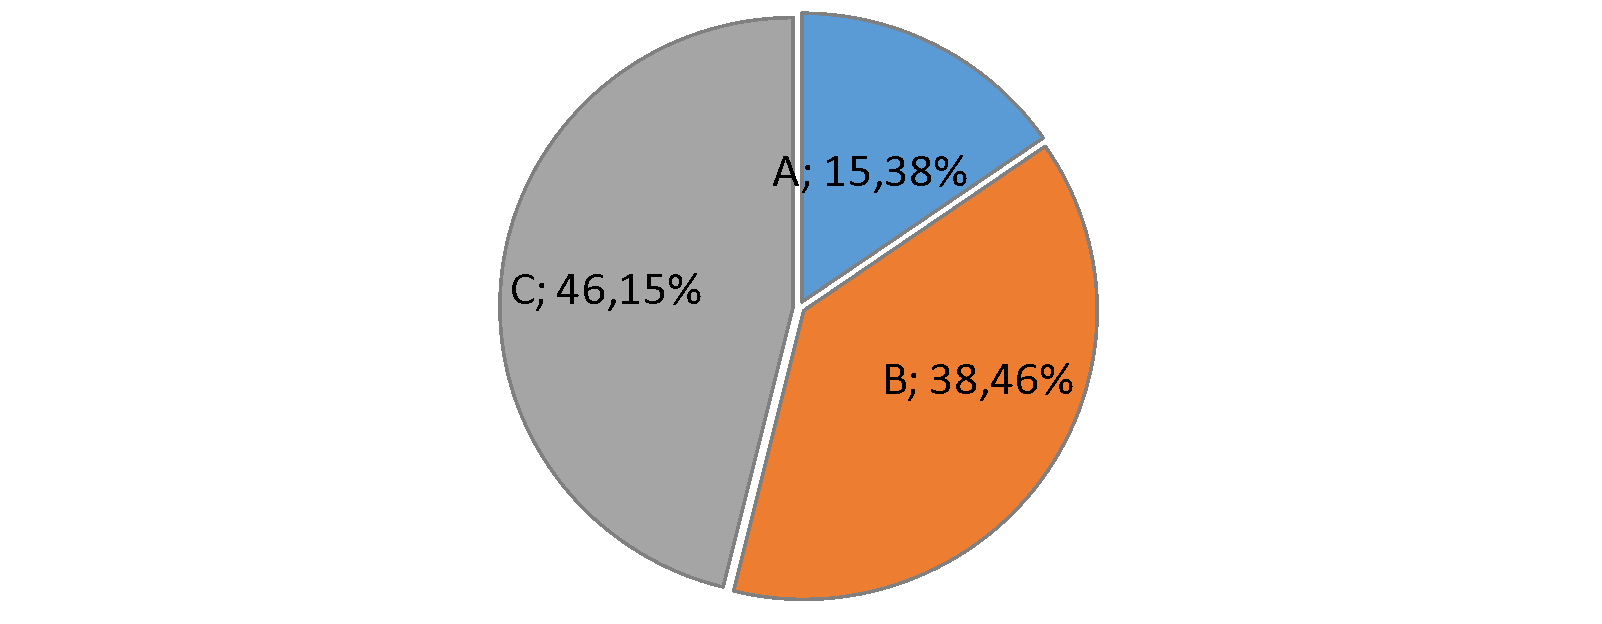
\includegraphics[width=4.6244in,height=1.8in,width=\textwidth]{monje-img2.png}
 \newline
\textbf{Figure 2. CEFR Proficiency level according to vocabulary size.}\newline
\textbf{ \ }
\end{styleNormali}


\begin{styleNormali}
\ \ \ Three native speakers participated in the study as a baseline group (2 female, 1 male; mean age = 24.8, \textit{SD} = 0.58). They all share a similar linguistic background, as they are linguistic majors and have a high command of two foreign languages, namely Spanish and French. Two participants are speakers of American English and the third participant is a speaker of Hiberno-English. For the purpose of this investigation, it is considered that VOT values do not differ as a function of language variety among native speakers, as they produce native-like values (i.e. above 60ms) (Lowenstein \& Nittrouer 2008). 
\end{styleNormali}


\begin{styleNormali}
\textbf{4.2 \ \ Procedure, tasks and stimuli}
\end{styleNormali}


\begin{styleNormali}
The factors found to influence VOT production mentioned above are taken into account in the present study (i.e. speaking style, vowel height and place of articulation). Speech samples were obtained for subsequent acoustic analysis. VOT was the segmental measure under scrutiny. Only voiceless stops in word-initial position and followed by a stressed vowel were included in the VOT analysis. Thirty-one word-initial voiceless stops produced three times by each of the 16 subjects (13 learners and three natives) at two\textbf{ }data collection times were measured.
\end{styleNormali}


\begin{styleNormali}
Participants were recorded in high quality sound-proof booths with the Audacity software and a \textit{Rode NT-1AX} microphone. They were instructed to complete two tasks: \ a carrier sentence task (isolated target words embedded in a carrier sentence – i.e. \textit{I say X, I say X now, I say X twice}) and a read aloud task (target words embedded in a text to be read continuously). The carrier-sentence/ read-aloud tasks were conceived to test participants’ VOT production of word-initial stops in stressed syllables. Participants were instructed to articulate the stimuli as clearly as possible in both tasks, but especially the target words present in the carrier-sentence task.
\end{styleNormali}


\begin{styleNormali}
Thirty-one monosyllabic words starting with a voiceless stop (/p, t, k/) were selected for the test. There were 29 distractors, resulting in a total of 60 words. Vowel height was taken into account, as it is an influencing factor in VOT production (Yavaş \& Wildermuth 2006). Of the 11 words starting with /p/, the stop was followed by a high vowel in five of the items (\textit{peach, pill, pear, pin, pig}) and by a low vowel in six of them (\textit{pub, pan, park, pup, part, pun}). Of the ten words starting with /t/, the stop was followed by a high vowel in five instances (\textit{tear, tip, two, ten, tent}) and by a low vowel in five of them (\textit{tan, tuck, touch, tart, toss}). As for the ten words starting with /k/, the stop was followed by a high vowel in five cases (\textit{key, could, kill, kilt, kit}) and by a low one in the remaining five (\textit{cod, card, cot, cap, cut}). See Table 2 for a complete stimuli list. Distractors are presented in Table 3. The 60 items were randomized and displayed in a PowerPoint presentation for the carrier-sentence task.
\end{styleNormali}


\begin{styleNormali}
\textbf{Table 2. Stimuli list for carrier sentence task.}
\end{styleNormali}


\begin{flushleft}
\tablehead{}
\begin{supertabular}{|m{0.70805985in}|m{0.75185984in}|m{0.70875984in}|m{0.8073598in}|m{0.66565984in}|m{0.6101598in}|}
\hline
\multicolumn{2}{|m{1.5386599in}|}{\centering /p/} &
\multicolumn{2}{m{1.5948598in}|}{\centering /t/} &
\multicolumn{2}{m{1.3545599in}|}{\centering /k/}\\\hline
\centering HV &
\centering LV &
\centering HV &
\centering LV &
\centering HV &
\centering\arraybslash LV\\\hline
\centering \textbf{peach} &
\centering \textbf{pub} &
\centering tear &
\centering \textbf{tan} &
\centering \textbf{key} &
\centering\arraybslash \textbf{cod}\\\hline
\centering \textbf{pill} &
\centering pan &
\centering tip &
\centering tuck &
\centering \textbf{could} &
\centering\arraybslash \textbf{card}\\\hline
\centering pear &
\centering \textbf{park} &
\centering \textbf{two} &
\centering touch &
\centering kill &
\centering\arraybslash cot\\\hline
\centering pin &
\centering pup &
\centering \textbf{ten} &
\centering \textbf{tart} &
\centering kilt &
\centering\arraybslash cap\\\hline
\centering pig &
\centering part &
\centering tent &
\centering toss &
\centering kit &
\centering\arraybslash cut\\\hline
\multicolumn{1}{m{0.70805985in}|}{} &
\centering pun &
\multicolumn{4}{m{3.0281599in}}{}\\\hhline{~-~~~~}
\end{supertabular}
\end{flushleft}
\begin{styleNormali}
\textbf{Table 3. Distractors for carrier sentence task.}
\end{styleNormali}


\begin{flushleft}
\tablehead{}
\begin{supertabular}{|m{0.6066598in}m{0.8080598in}m{0.8073598in}m{0.70875984in}m{0.6101598in}m{0.71085984in}|}
\hline
\centering bark &
\centering group &
\centering Bart &
\centering dart &
\centering beach &
\centering\arraybslash Dutch\\
\centering duck &
\centering do &
\centering bun &
\centering ghee &
\centering grew &
\centering\arraybslash gap\\
\centering God &
\centering big &
\centering dent &
\centering bear &
\centering dear &
\centering\arraybslash ban\\
\centering Dan &
\centering den &
\centering got &
\centering doss &
\centering guilt &
\centering\arraybslash bin\\
\centering Bill &
\centering good &
\centering guard &
\centering gut &
\centering dip &
\\\hline
\end{supertabular}
\end{flushleft}
\begin{styleNormali}
\newline
 \ \ The second task was a text designed to be read aloud naturally with the purpose of taking into account the effect of speaking style. In order to do so, 12 items starting with a voiceless stop were selected (in bold in Table 2), four of which begin with /p/ (\textit{pill, peach, pub, park}), four with /t/ (\textit{two, ten, tan, tart}) and four with /k/ (\textit{keys, could, cod, card}). In 6 items, the stop was immediately followed by a high vowel (\textit{key, ten, could, pill, two, peach}) and in the other 6, the stop was immediately followed by a low vowel (\textit{tan, park, pub, cod, tart, card}). The text was printed and physically handed to the participants for them to read aloud. 
\end{styleNormali}


\begin{styleNormali}
The tasks were administered in two different orders with the purpose of counterbalancing task effects. In Order 1 the carrier sentence task was performed first, whereas in Order 2, participants started by reading the text. They were asked to read the text as naturally as possible. Additionally, at T1 the learners completed the Carlet-SALA questionnaire, a language background questionnaire that resulted from the combination of the questionnaire used in Carlet (2017) and the SALA questionnaire on SA conditions. They did so once they had performed the task. Lastly, they performed the vocabulary size test (Meara 2005; Meara \& Miralpeix 2006) at T2.
\end{styleNormali}


\begin{listWWNumiileveli}
\item 
\begin{styleNormali}
\textbf{Results and discussion}
\end{styleNormali}

\end{listWWNumiileveli}
\begin{listWWNumiileveli}
\item 
\setcounter{listWWNumiilevelii}{0}
\begin{listWWNumiilevelii}
\item 
\begin{styleNormali}
\textbf{\ \ Research Question 1}
\end{styleNormali}

\end{listWWNumiilevelii}
\end{listWWNumiileveli}
\begin{styleNormali}
Given the sample size, Wilcoxon signed-rank nonparametric tests for related samples were performed. As shown in Table 4 and Figure 3, participants displayed slightly longer VOT values at T2 than at T1. However, the 2-month FI period immediately following a 3-month long SA period was found to have no statistically significant effect on the VOT production of voiceless plosive consonants (\textit{z }= 0.384, \textit{N }= 13, \textit{p }= .3505, one-tailed).\textbf{ \ }
\end{styleNormali}


\begin{styleNormali}
\ \ Similar results were also obtained when analysing the two tasks separately. As can be seen in Table 4 and Figure 3, participants displayed slightly longer VOT values at T2 than at T1 for both tasks. A further Wilcoxon-test was run in order to reveal whether this difference reached statistical significance. Again, the 2-month FI period immediately following a 3-month long SA term was found to have no statistically significant effect on the VOT production of voiceless plosive consonants in either the text (\textit{z} = 0.314, \textit{N }= 13, \textit{p} = .3765, one-tailed) or the carrier sentence task (\textit{z} = 0.454, \textit{N }= 13, \textit{p} = .325, one-tailed). 
\end{styleNormali}


\begin{styleNormali}
\textbf{Table 4. Mean VOT measurements (ms) at both testing times (T1, T2).}
\end{styleNormali}


\begin{flushleft}
\tablehead{}
\begin{supertabular}{|m{1.6552598in}m{1.2268599in}m{1.4844599in}m{1.5663599in}|}
\hline
\multicolumn{1}{|m{1.6552598in}|}{\centering \textbf{~}} &
\multicolumn{2}{m{2.79006in}|}{\centering \textbf{Non-native speakers}} &
\centering\arraybslash \textbf{Native English speakers}\\\hline
\multicolumn{1}{|m{1.6552598in}|}{} &
\multicolumn{1}{m{1.2268599in}|}{\centering \textbf{T1}\par

\centering \textbf{ms \ \ \ (sd)}} &
\multicolumn{1}{m{1.4844599in}|}{\centering \textbf{T2}\par

\centering \textbf{ms \ \ \ (sd)}} &
\centering\arraybslash \textbf{ms \ \ \ (sd)}\\\hline
\centering \textbf{Both tasks} &
\centering 51.05 (20.39) &
\centering 51.54 (18.13) &
\centering\arraybslash 65.47 (24.94)\\\hline
\centering \textbf{Words} &
\centering 54.93 (23.55) &
\centering 55.07 (20.13) &
\centering\arraybslash 67.96 (29.87)\\\hline
\end{supertabular}
\end{flushleft}
\begin{styleNormali}
  [Warning: Image ignored] % Unhandled or unsupported graphics:
%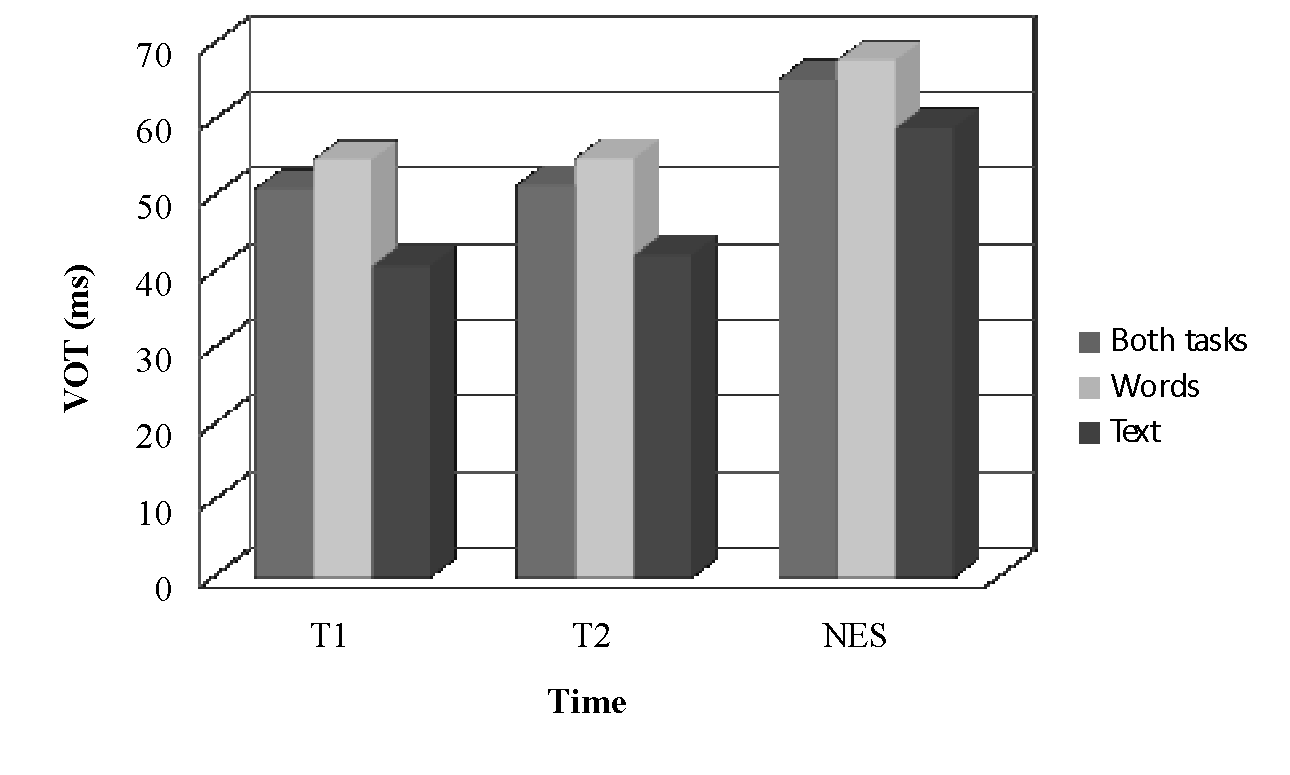
\includegraphics[width=5in,height=3in,width=\textwidth]{monje-img3.png}
 
\end{styleNormali}


\begin{styleNormali}
\textbf{Figure 3. Mean VOT measurements (ms) at both testing times (T1, T2).}
\end{styleNormali}


\begin{styleNormali}
These results may be interpreted as follows: The lack of explicit focus on L2 phonology in the FI participants received might account for the fact that the slight lengthening of VOT values displayed at T2 failed to reach statistical significance. This view is supported by those studies stressing the need for explicit attention to L2 phonology in FI for the improvement of L2 production accuracy (Darcy et al. 2012; Gordon \& Darcy 2012; Calvo Benzies 2014).
\end{styleNormali}


\begin{styleNormali}
\ \ Hence, the answer to our research question is that a 2-month FI period preceded by a 3-month long SA term has no statistically significant effect on the VOT production of voiceless plosive consonants. Our hypothesis has not been confirmed as results are not significant. However, we have obtained a numerical tendency towards the native-like model in the VOTs of plosive consonants in initial position. Importantly, the native group always produced longer VOTs than the non-native participants. The shorter VOT found for non-NES confirmes the SLM’s prediction and finding that EFL learners produce intermediate VOT values between their L1 and their L2 (Flege 1987; 1995; Flege et al. 1998; Reis \& Nobre-Oliveira 2007; Yavaş 2007; Mora 2008; Wrembel 2011; 2013; Schwartzhaupt \& Alves 2014; Alves \& Zimmer 2015). As explained by the SLM, learners perceive the L2 sounds in relation to their pre-existing L1 categories. Therefore, this model accounts for the intermediate VOT values produced by our participants, whose interlanguage is in the process of moving towards the target language values. Importantly, the SLM does not predict that learners can completely attain native-like VOT values. \ It must be noted, however, that no statistical tests were run comparing both groups due to the low number of participants. For this reason, the native speakers served the present investigation solely as a baseline group.
\end{styleNormali}


\begin{listWWNumiileveli}
\item 
\setcounter{listWWNumiilevelii}{0}
\begin{listWWNumiilevelii}
\item 
\begin{styleNormali}
\textbf{Sub-Research Question 1.1}
\end{styleNormali}

\end{listWWNumiilevelii}
\end{listWWNumiileveli}
\begin{styleNormali}
In order to assess whether VOT productions differed as a function of proficiency level (assessed with the lexical test), participants were divided into two proficiency groups (high level group, low level group). Participants with A and B proficiency levels were considered the lower level group, whereas participants with a C level made up the high-level group. Data gathered at both times were averaged and are displayed in Table 5 and in Figure 4. Given the small sample size of each individual group, the results concerning this sub-research question were not submitted to statistical analyses. Group differences will thus be discussed in terms of numerical differences in the descriptive statistics.
\end{styleNormali}


\begin{styleNormali}
\ \ \ \textbf{Table 5. Mean VOT measurements (ms) as a function of proficiency level.}
\end{styleNormali}


\begin{flushleft}
\tablehead{}
\begin{supertabular}{|m{1.5045599in}|m{1.8893598in}|m{2.42056in}|}
\hline
\multicolumn{1}{|m{1.5045599in}}{\centering \textbf{Participants}} &
\centering \textbf{T1}\par

\centering \textbf{ms \ \ \ \ sd} &
\textbf{\ \ \ \ \ \ \ \ \ \ \ \ \ \ \ \ \ \ \ \ \ \ \ \ \ \ \ \ \ \ \ \ T2}

\centering\arraybslash \textbf{ms \ \ \ \ sd}\\\hline
\centering \textbf{Native English speakers} &
\multicolumn{2}{m{4.38866in}|}{\ \ \ \ \ \ \ \ \ \ \ \ \ \ \ \ 65.47 (24.94)}\\\hline
\centering \textbf{High Level Group} &
\centering 60.11 (21.26) &
\centering\arraybslash 55.83 (16.56)\\\hline
\centering \textbf{Low Level Group} &
\centering 43.27 (20.12) &
\centering\arraybslash 47.87 (18.96)\\\hline
\end{supertabular}
\end{flushleft}
\begin{styleNormali}
  [Warning: Image ignored] % Unhandled or unsupported graphics:
%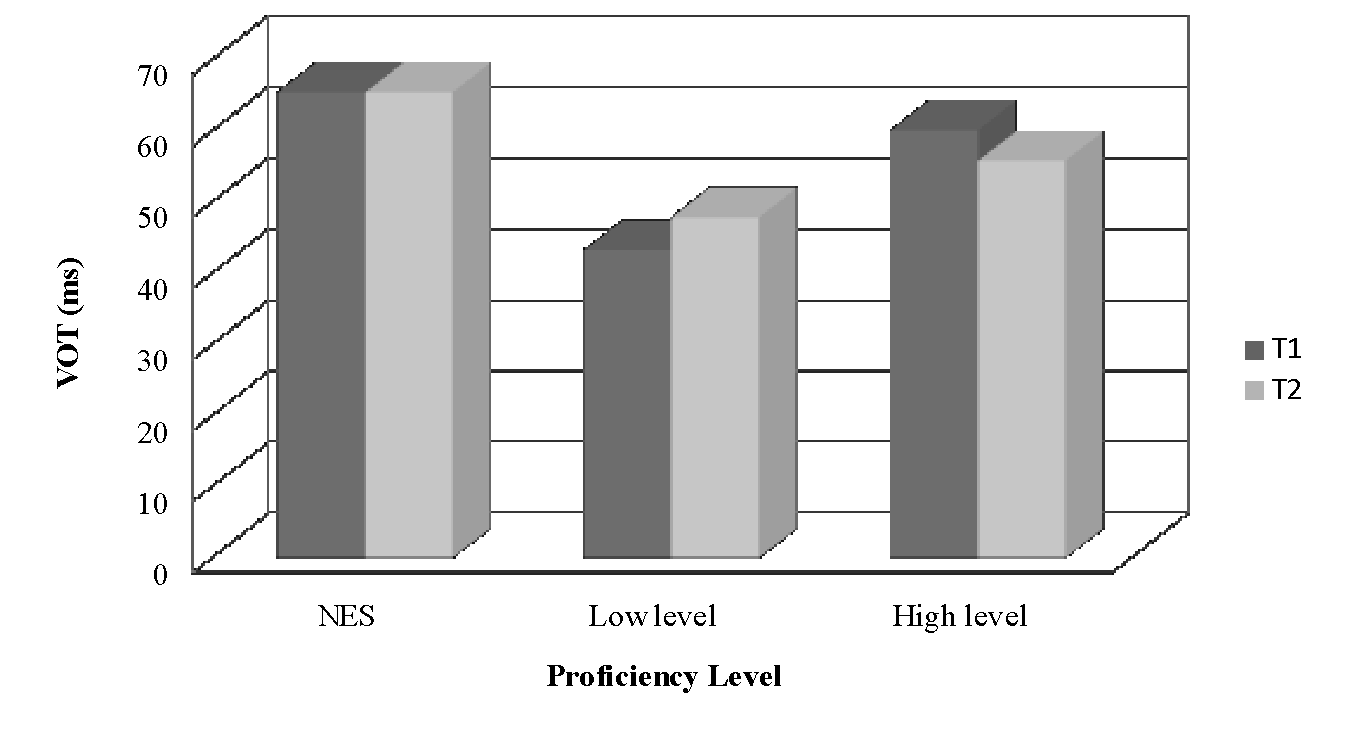
\includegraphics[width=5.9043in,height=3.2402in,width=\textwidth]{monje-img4.png}
 
\end{styleNormali}


\begin{styleNormali}
\textbf{Figure 4. Mean VOT measurements (ms) as a function of proficiency level.}
\end{styleNormali}


\begin{styleNormali}
Interestingly, it can be observed in Table 5 \ that the high-level group obtained numerically higher and more native-like VOT values than the low-level group at the outset of the study, that is, after the SA period. This result might point towards a tendency of language experience to have a potential impact on L2 phonological category learning, as predicted by the SLM. Along these lines, the more advanced group experienced stronger effects of category learning than the least experienced group, as a result of the SA period. 
\end{styleNormali}


\begin{styleNormali}
\ \ Looking more closely at the performance of both groups over time, the lower level group shows the largest improvement (43.27\% to 47.87\%). In fact, the higher proficiency group experiences a slight numerical decrease in VOT (60.11\% to 55.83\%). These results point to a tendency for improvement for the lower level group, while the tendency points in the opposite direction for the high-level group. These results, even though drawn from a small sample, may suggest that the high-level group had reached their ceiling VOT values during the SA period, whereas the lower level group still had room for improvement. A potential reason for this is that the likely L2 categories formed by the high-level group for the target segments are more robust than those of the low-level group. Therefore, the FI period following the SA might have been more effective in enhancement of L2 VOT production for the low-level group than for their more advanced counterpart. This numerical tendency found in our data is in line with Collentine’s (2009) notion of a \textit{threshold level.}
\end{styleNormali}


\begin{styleNormali}
\ \ Thus, it can be said that proficiency level seems to play a significant role in the VOT production of English plosive consonants in initial stressed position by Catalan/Spanish EFL learners, at least as far as the effects of an FI period following a SA period are concerned. However, given the small sample size and the lack of inferential statistical analysis, this study should be seen as mainly exploratory.
\end{styleNormali}


\begin{listWWNumiileveli}
\item 
\setcounter{listWWNumiilevelii}{0}
\begin{listWWNumiilevelii}
\item 
\begin{styleNormali}
\textbf{Sub-Research Question 1.2.}
\end{styleNormali}

\end{listWWNumiilevelii}
\end{listWWNumiileveli}
\begin{styleNormali}
In order to explore whether the VOT values obtained significantly differ as a function of task type, a Wilcoxon-test was performed on the non-native data. As shown in Table 6 and Figure 5, for both the non-native and the native groups, the VOT durations produced when reading the text were significantly shorter than those obtained during the carrier sentence task at both times (\textit{z }= 2.830, \textit{N }= 13, \textit{p }= .0025, one-tailed) as well as at T1 (\textit{z }= 2.621, \textit{N }= 13, \textit{p }= .0045, one-tailed) and at T2 (\textit{z }= 2.900, \textit{N }= 13, \textit{p }= .002, one-tailed). 
\end{styleNormali}


\begin{styleNormali}
\textbf{Table 6. Mean VOT measurements (ms) as a function of task (text vs. words).}
\end{styleNormali}


\begin{flushleft}
\tablehead{}
\begin{supertabular}{m{0.5872598in}m{1.1018599in}m{1.4955599in}|m{1.2011598in}|m{1.5705599in}}
 &
\multicolumn{3}{m{3.95606in}|}{\centering \textbf{Non-native speakers}} &
\centering\arraybslash \textbf{Native English speakers}\\\hline
 &
\centering \textbf{T1}\par

\centering \textbf{ms \ \ \ \ sd} &
\centering \textbf{T2}\par

\centering \textbf{ms \ \ \ \ sd} &
\centering \textbf{T1+T2}\par

\centering \textbf{ms \ \ \ \ sd} &
\centering\arraybslash \textbf{ms \ \ \ \ sd}\\\hline
\multicolumn{1}{m{0.5872598in}|}{\centering \textbf{Words}} &
\multicolumn{1}{m{1.1018599in}|}{\centering 54.93 \ (23.55)} &
\centering 55.07 (20.13) &
\centering 55.00 (20.91) &
\centering\arraybslash 67.96 (29.87)\\\hline
\multicolumn{1}{m{0.5872598in}|}{\centering \textbf{Text}} &
\multicolumn{1}{m{1.1018599in}|}{\centering 40.99 (14.55)} &
\centering 42.40 (13.98) &
\centering 41.69 (13.28) &
\centering\arraybslash 59.06 (13.54)\\\hline
\end{supertabular}
\end{flushleft}
\begin{styleNormali}
  [Warning: Image ignored] % Unhandled or unsupported graphics:
%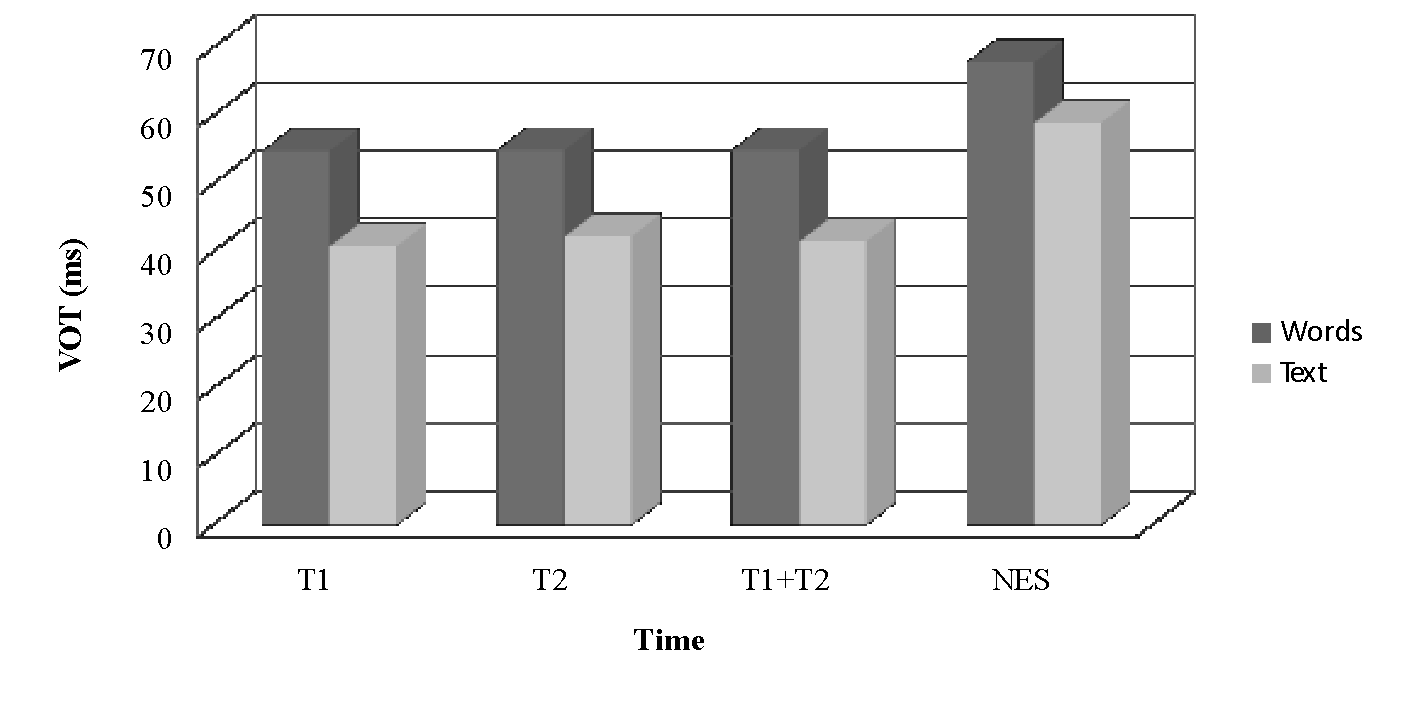
\includegraphics[width=5.9362in,height=3.0244in,width=\textwidth]{monje-img5.png}
 
\end{styleNormali}


\begin{styleNormali}
\textbf{Figure 5. Mean VOT measurements (ms) as a function of task (text vs. words).}
\end{styleNormali}


\begin{styleNormali}
The results presented here suggest that speaking style significantly affects the VOT production of Catalan/Spanish learners of English, answering sub-research question 1.2. Despite the lack of statistical differences between the native and non-native groups, the numerical values obtained from the natives suggest that speaking style affected both our groups of participants similarly. Our hypothesis is thus confirmed. Our data support Labov’s (1972) original idea that speaking style does have an effect on pronunciation and more specifically on VOT production, as also found by Mora (2008) and Bach (2012), confirming that in continuous speech, VOT values tend to decrease, whereas they tend to increase when produced in (quasi-)isolation. 
\end{styleNormali}


\begin{listWWNumiileveli}
\item 
\setcounter{listWWNumiilevelii}{0}
\begin{listWWNumiilevelii}
\item 
\begin{styleNormali}
\textbf{Sub-Research Question 1.3.}
\end{styleNormali}

\end{listWWNumiilevelii}
\end{listWWNumiileveli}
\begin{styleNormali}
With the purpose of determining whether there are differences in the VOT values as a function of the height of the vowel, another Wilcoxon-test was conducted. As observed in Table 7 and Figure 6, VOTs produced preceding a high vowel were longer than those followed by a low vowel both for the native and the non-native speakers. The test on the non-native speaker data revealed that this difference did reach statistical significance between the VOT values of high and low vowels (\textit{z }= 3.180, \textit{N }= 13, \textit{p}= .0005, one-tailed).
\end{styleNormali}


\begin{styleNormali}
\textbf{Table 7. Mean VOT measurements (ms) as a function of vowel height averaged across time (T1+T2).}
\end{styleNormali}


\begin{flushleft}
\tablehead{}
\begin{supertabular}{|m{1.3962599in}|m{1.7927599in}|m{1.4969599in}|}
\hline
 &
\centering \textbf{Non-native speakers}\par

\centering \textbf{ms \ \ \ \ sd} &
\centering \textbf{Native English speakers}\par

\centering\arraybslash \textbf{ms \ \ \ \ sd}\\\hline
\centering \textbf{High Vowel} &
\centering 56.52 (18.04) &
\centering\arraybslash 71.51 (25.75)\\\hline
\centering \textbf{Low Vowel} &
\centering 46.25 (18.96) &
\centering\arraybslash 59.72 (24.18)\\\hline
\end{supertabular}
\end{flushleft}
\begin{styleNormali}
  [Warning: Image ignored] % Unhandled or unsupported graphics:
%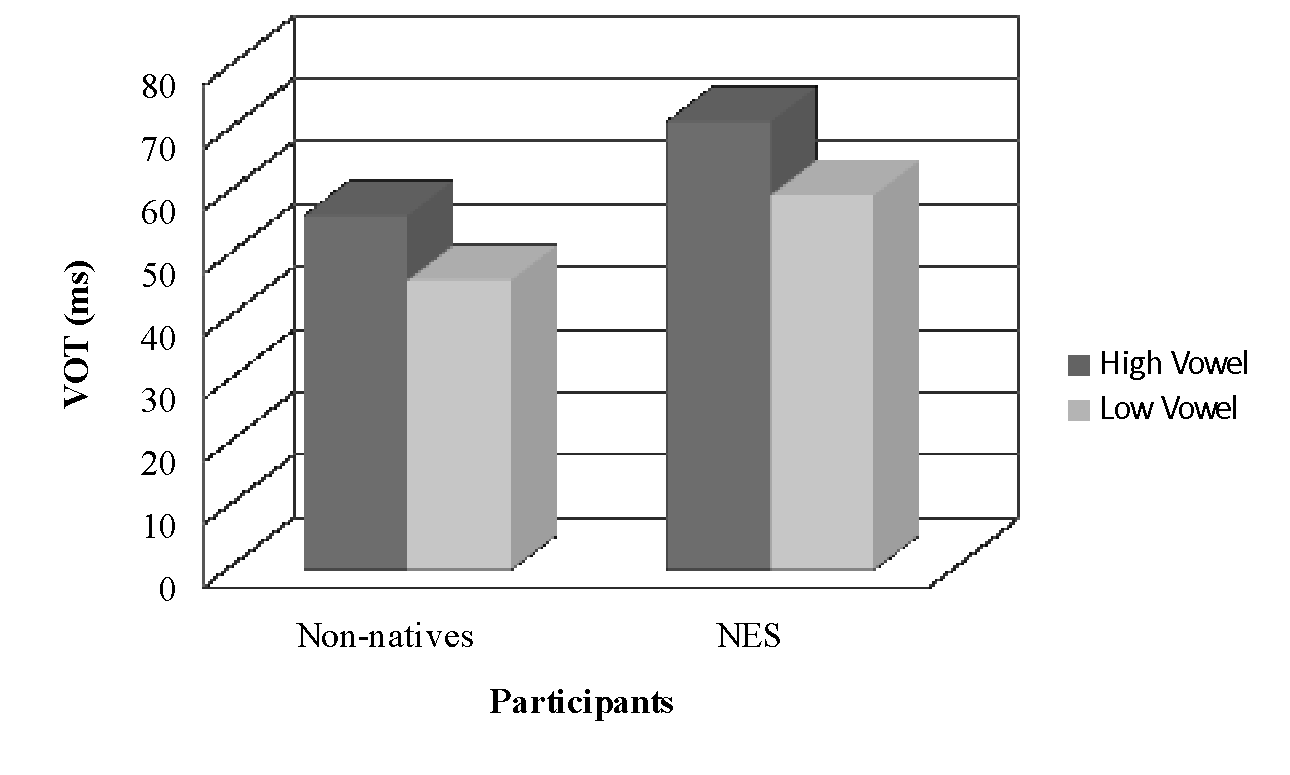
\includegraphics[width=5in,height=3in,width=\textwidth]{monje-img6.png}
 \newline
\textbf{Figure 6. Mean VOT measurements (ms) as a function of vowel height averaged across time (T1+T2).}
\end{styleNormali}


\begin{styleNormali}
These results suggest that vowel height does have a significant effect on VOT production of Catalan/Spanish learners of English, answering sub-research question 1.3. Interestingly, a similar pattern was observed for the native speakers. The hypothesis formulated regarding this sub-RQ is confirmed by the data and in line with Flege et al. (1998) and Yavaş and Wildermuth’s (2006) findings that vowel height does influence VOT production. 
\end{styleNormali}


\begin{listWWNumiileveli}
\item 
\setcounter{listWWNumiilevelii}{0}
\begin{listWWNumiilevelii}
\item 
\begin{styleNormali}
\textbf{Sub-Research Question 1.4.}
\end{styleNormali}

\end{listWWNumiilevelii}
\end{listWWNumiileveli}
\begin{styleNormali}
To determine whether VOT values differed as a function of place of articulation, three Wilcoxon-tests were run on the data obtained from non-native speakers. As shown by Table 8 and Figure 7, /k/ displayed the longest VOT values, with /t/ in the second place and /p/ having triggered the shortest durations for the non-native group. However, natives produced slightly longer VOTs for /t/ than for /k/. In turn, VOT values for /p/ were the shortest for this group.
\end{styleNormali}


\begin{styleNormali}
\textbf{Table 8. Mean VOT measurements (ms) as a function of place of articulation averaged across time (T1+T2).}
\end{styleNormali}


\begin{flushleft}
\tablehead{}
\begin{supertabular}{|m{1.5566599in}|m{1.1025599in}|m{1.6927599in}|m{1.6927599in}|}
\hline
 &
\textbf{\ \ \ \ \ \ \ \ \ \ \ \ K}

\centering \textbf{ms \ \ \ \ sd} &
\centering \textbf{T}\par

\centering \textbf{ms \ \ \ \ sd} &
\centering \textbf{\ \ P}\par

\centering\arraybslash \textbf{ms \ \ \ \ sd}\\\hline
\centering \textbf{Non-native speakers} &
\centering 61.62 (20,17) &
\centering 57.50 (22.09) &
\centering\arraybslash 35.78 (15.26)\\\hline
\centering \textbf{Native English speakers} &
\centering 70.44 (24.68) &
\centering 72.79 (22.81) &
\centering\arraybslash 54.01 (27.28)\\\hline
\end{supertabular}
\end{flushleft}
\begin{styleNormali}
[Warning: Draw object ignored]
\end{styleNormali}


\begin{styleNormali}
  [Warning: Image ignored] % Unhandled or unsupported graphics:
%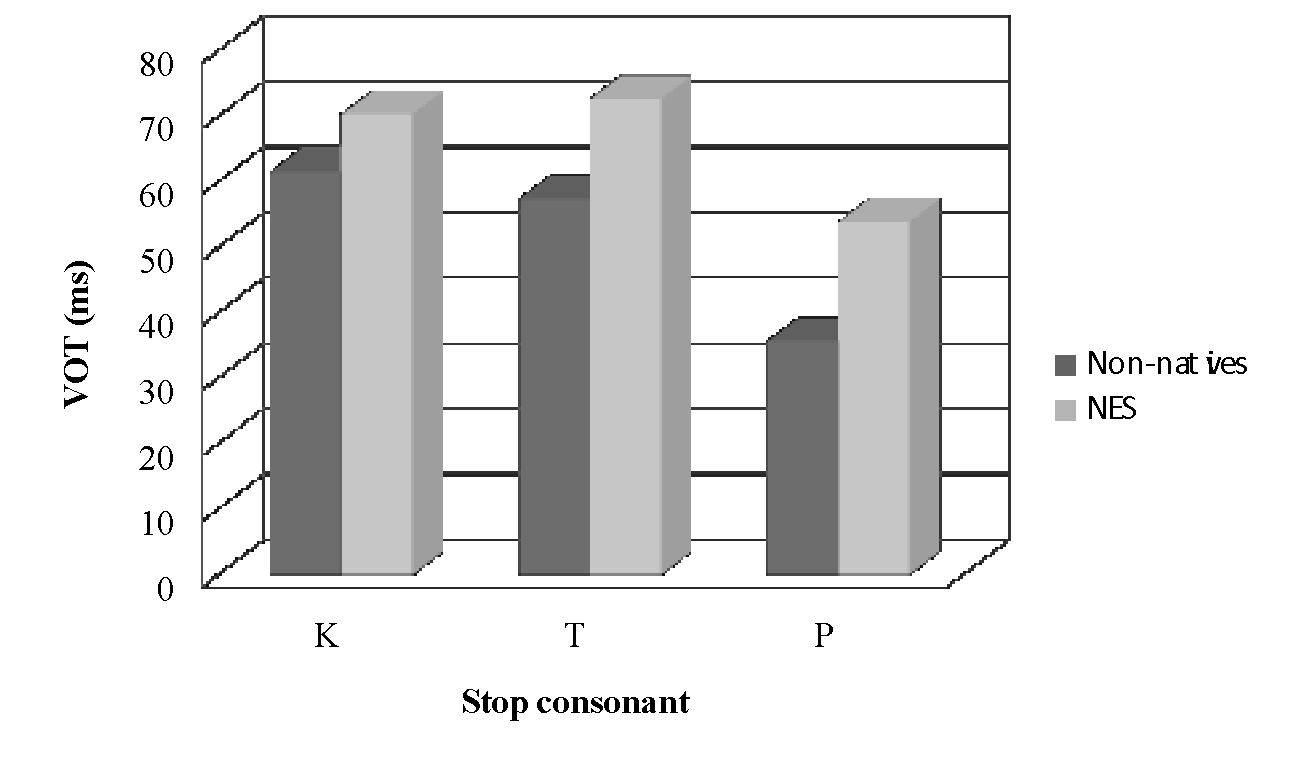
\includegraphics[width=5in,height=3in,width=\textwidth]{monje-img7.png}
 
\end{styleNormali}


\begin{styleNormali}
\textbf{Figure 7. Mean VOT measurements (ms) as a function of place of articulation averaged across time (T1+T2).}
\end{styleNormali}


\begin{styleNormali}
The test revealed that VOT values obtained for /p/ were significantly different from those obtained for /k/ (\textit{z} = 3.180, \textit{N }= 13, \textit{p} = .0005, one-tailed) and for /t/ (\textit{z }= 3.180, \textit{N }= 13, \textit{p }= .0005, one-tailed), respectively. However, VOT values obtained for /k/ and /t/ were not significantly different from one another (\textit{z }= 1.223, \textit{N }= 13, \textit{p }= .1105, one-tailed). \ 
\end{styleNormali}


\begin{styleNormali}
\ \ The relative similarity of VOT values for /k/ and /t/ might be explained by the fact that they are quite similar in native speakers as well. Moreover, according to Alves \& Zimmer (2015), aspiration is a cue that learners pay attention to, which might explain why the VOT values for /k/ and /t/ did not to reach statistical significance in the present study.\textbf{ }Specifically, it is more salient in some places of articulation than in others. This seems to indicate that our participants are in the process of creating L2 categories for the target segments, as their performance shows certain similarities with that of the baseline group. Although their VOT durations never reach those produced by the natives, as predicted by the SLM, the initial hypothesis that place of articulation affects VOT (Yavaş \& Wildermuth 2006) is confirmed.
\end{styleNormali}


\begin{listWWNumiileveli}
\item 
\begin{styleNormali}
\textbf{Summary and Conclusions}
\end{styleNormali}

\end{listWWNumiileveli}
\begin{styleNormali}
The present study aimed at making a contribution to the SALA project by providing a study not undertaken before. Moreover, it sought to reduce the present research gap in the field of L2 phonology acquisition during SA in combination with a subsequent FI period. It sought to examine and measure the effects of a 2-month FI period, with no specific training in the learners’ L2 phonological abilities, preceded by a 3-month long SA term, on the VOT production by Catalan/Spanish EFL learners.
\end{styleNormali}


\begin{styleNormali}
\ \ Results revealed that a 2-month FI period preceded by a 3-month long SA term undergone by our participants had no statistically significant effects on their VOT production of English voiceless plosive consonants, although a tendency towards improvement was observed. Such findings might be due to the limited statistical power of this exploratory study, but they may also lead one to reflect on the absence of explicit instruction on L2 phonology which characterises most FI. \ We are thus led to wonder whether an FI with explicit instruction on L2 phonology would have a positive effect on L2 phonological acquisition in EFL learners.
\end{styleNormali}


\begin{styleNormali}
\ \ Moreover, proficiency level might play a role on VOT production, given that the high level group displayed higher values than the low level one, although this was not statistically confirmed. In addition, ceiling effects were found in the advanced group, whereas the lower level group seemed to have more room for improvement. These findings must tentatively be taken as tendencies. On the other hand, speaking style, vowel height, and place of articulation do significantly affect VOT production of voiceless plosives by Catalan/Spanish learners. The native group displayed a similar numerical pattern, which indicates that these three independent factors affect both groups in a similar way. However, natives always produce higher VOT values for English voiceless stops, confirming that EFL learners tend to produce intermediate VOT values between their L1 and their L2 for the same consonants. As for speaking style, words in (quasi-)isolation (carrier sentence task) displayed significantly higher values than those produced in continuous speech (read aloud task). We might interpret these results by stating that the more attention is paid when uttering words, the more likely the sounds produced are to be clearly articulated. As for vowel height, VOT values produced before a high vowel were significantly longer than those produced preceding a low vowel. Finally, concerning place of articulation, VOTs for /k/ displayed the highest values, with /t/ in the second place and values for /p/ being the shortest. It must be stressed that only the /k/ vs. /t/ comparison failed to reach statistical significance. The results concerning place of articulation can be understood through the SLM. Our participants seem to be in the process of creating L2 categories for voiceless stops, as they performed similarly to the native group regarding the lack of difference between /k/ and /t/. This suggests that aspiration is more salient in some places of articulation than in others (Alves \& Zimmer, 2015). 
\end{styleNormali}


\begin{listWWNumiileveli}
\item 
\begin{styleNormali}
\textbf{Limitations and directions for prospective research}
\end{styleNormali}

\end{listWWNumiileveli}
\begin{styleNormali}
In this final section, we identify some of the limitations of the current study and highlight directions for future research. When work on this study started, it was no longer possible to test participants prior to their experience abroad, and thus VOT measurements before SA could not be obtained. The reason is that informants were already abroad by data collection T1. Hence, all collected data were gathered only after the SA period, so the obtained VOTs cannot be contrasted against those prior to SA, which would presumably have provided valuable information as for the learners’ VOT departure values.
\end{styleNormali}


\begin{styleNormali}
One other issue is the measurement of proficiency level. Testing should have been conducted at both data collection times, and not only at T2. Time constraints prevented this from happening. 
\end{styleNormali}


\begin{styleNormali}
In addition, the number of participants was low, both for the non-native and the native groups. This prevented us from drawing general conclusions and accentuates the fact that conclusions related to our population must be taken with caution. Finally, the native speakers who served as a baseline group are not monolingual, so their VOT values might have been influenced by other languages. However, all of them are late bilinguals.
\end{styleNormali}


\begin{styleNormali}
\ \ Despite the lack of statistical reliability for some of the tendencies we found, they leave a door open to prospective research, namely with a larger population so that more robust claims can be made. A further study should measure the effects of a post-stay-abroad FI period including either explicit instruction on L2 phonology or L2 phonetic training and focusing either on the VOT of English stops or on other relevant acoustic cues.
\end{styleNormali}


\begin{styleNormali}
\textbf{References}
\end{styleNormali}


\begin{styleNormali}
Abramson, Arthur S. \& Lisker, Leigh. 1964. A cross-language study of voicing in initial stops: Acoustical measurements. \textit{Word }20\textit{.} 384–422.
\end{styleNormali}


\begin{styleNormali}
Abramson, Arthur S. \& Lisker, Leigh. 1967. The voicing dimension: Some experiments in comparative phonetics. In \textit{Proceedings of the 6th international congress of phonetic sciences,} 9–15.\textbf{ }Prague: Academia.
\end{styleNormali}


\begin{styleNormali}
Alves, Ubiratã Kickhöfel \& Zimmer, Márcia Cristina. 2015. Perception and production of English VOT patterns by Brazilian learners: The role of multiple acoustic cues in a DST perspective. \textit{Alfa: Revista de Linguística (São José do Rio Preto} 59(1). 157–180.
\end{styleNormali}


\begin{styleNormali}
Archibald, John. 2005. Second language phonology as redeployment of L1 phonological knowledge. \textit{The Canadian Journal of Linguistics }50. 285–314.
\end{styleNormali}


\begin{styleNormali}
Avello, Pilar. 2010. The effect of study abroad on Catalan/Spanish bilinguals’ production of English /i:-[26A?]/ and /æ-[28C?]/ contrasting pairs. (Paper presented at the 6th international conference on language acquisition - CIAL, Universitat de Barcelona, Spain.)
\end{styleNormali}


\begin{styleNormali}
Bach, Ocke-Schwen. 2012. \textit{Coexistence of phonetic systems in Danish/English bilinguals: A study of the production of VOT categories. }Aarhus: University of Aarhus. (M.A. dissertation.)
\end{styleNormali}


\begin{styleNormali}
Brecht, Richard. \& Davidson, Dan. \& Ginsberg, Ralph. 1995. Predictors of foreign language gain during study abroad. In Barbara Freed (ed.), \textit{Second language acquisition in a study abroad context}, 37–66. Amsterdam: Benjamins.
\end{styleNormali}


\begin{styleNormali}
Calvo Benzies, Yolanda Joy. 2014. The teaching of pronunciation in Spain: Students´ and teachers{\textquotesingle} views. In Tania Pattison (ed.), \textit{IATEFL 2013 Liverpool Conference Selections}, 106–108. Faversham, UK: IATEFL.
\end{styleNormali}


\begin{styleNormali}
Calvo Benzies, Yolanda Joy. 2016. \textit{The teaching and learning of English pronunciation in Spain. An analysis and appraisal of students’ and teachers’ views and teaching materials.} Santiago: University of Santiago de Compostela. (Doctoral dissertation.) 
\end{styleNormali}


\begin{styleNormali}
Carlet, Angélica. 2017. \textit{L2 perception and production of English consonants and vowels by Catalan speakers: The effects of attention and training task in a cross-training study.} Barcelona: Universitat Autònoma de Barcelona. (Doctoral dissertation.)
\end{styleNormali}


\begin{styleNormali}
Cho, Taehong \& Ladefoged, Peter. 1999. Variation and universals in VOT: Evidence from 18 languages. \textit{Journal of Phonetics }27\textit{. }207–229. 
\end{styleNormali}


\begin{styleNormali}
Collentine, Joseph. 2009. Study abroad research: Findings, implications and future directions. In Michael H. Long \& Catherine J. Doughty (eds.), \textit{The handbook of language teachin}g\textit{,} 218–233. Malden, MA: Blackwell. 
\end{styleNormali}


\begin{styleNormali}
Dalton, Christiane \& Seidlhofer, Barbara. 1994. \textit{Pronunciation}. Oxford: Oxford University Press.
\end{styleNormali}


\begin{styleNormali}
Darcy, Isabelle \& Ewert, Doreen \& Lidster, Ryan. 2012. Bringing pronunciation instruction back into the classroom: An ESL Teachers{\textquotesingle} pronunciation {\textquotedbl}toolbox{\textquotedbl}. In John Levis \& Kimberly LeVelle (eds.), \textit{Proceedings of the 3rd pronunciation in second language learning and teaching conference}, 93–108. Ames, IA: Iowa State University.
\end{styleNormali}


\begin{styleNormali}
DeKeyser, Robert. 2007. Skill acquisition theory. In Bill VanPatten \& Jessica Williams (eds.), \textit{Theories in second language acquisition: An introduction,} 97–114. Mahwah, NJ: Lawrence Erlbaum.
\end{styleNormali}


\begin{styleNormali}
Derwing, Tracey. 2010. Utopian goals for pronunciation teaching. In John Levis \& Kimberly LeVelle (eds.), \textit{Proceedings of the 1st pronunciation in second language learning and teaching conference}, 24–37. Ames, IA: Iowa State University.
\end{styleNormali}


\begin{styleNormali}
Derwing, Tracey \& Foote, Jennifer Ann. 2011. 2010 national survey of pronunciation teaching: Deja vu. (Paper presented at the American Association for Applied Linguistics, Chicago, IL.) 
\end{styleNormali}


\begin{styleNormali}
Díaz-Campos, Manuel. 2004. Context of learning in the acquisition of Spanish second language phonology. \textit{Studies in Second Language Acquisition }26. 249–273.
\end{styleNormali}


\begin{styleNormali}
Flege, James Emil. 1987. The production of {\textquotesingle}new{\textquotesingle} and {\textquotesingle}similar{\textquotesingle} phones in a foreign language: Evidence for the effect of equivalent classification. \textit{Journal of Phonetics }15. 47–65.
\end{styleNormali}


\begin{styleNormali}
Flege, James Emil. 1995. Second language speech learning theory, findings, and problems. In Strange, W. (ed.), \textit{Speech perception and linguistic experience: Issues in cross-language research}, 233–277. Timonium, MD: York Press.
\end{styleNormali}


\begin{styleNormali}
Flege, James Emil. \& Frieda, Elaina M. 1997. Amount of native-language (L1) use affects the pronunciation of an L2. \textit{Journal of Phonetics} 25. 169–186.
\end{styleNormali}


\begin{styleNormali}
Flege, James Emil \& Frieda, Elaina M. \& Walley, Amandas C. \& Randazza, Lauren A. 1998. Lexical factors and segmental accuracy in second language speech production. \textit{Studies in Second Language Acquisition }20(2). 155–187.
\end{styleNormali}


\begin{styleNormali}
Foote, Jennifer Ann \& Holtby, Amy K. \& Derwing, Tracey M. 2011. Survey of pronunciation teaching in adult ESL programs in Canada, 2010. \textit{TESL Canada Journal }29(1). 1–22.
\end{styleNormali}


\begin{styleNormali}
Gordon, James. \& Darcy, Isabelle. 2012. The development of comprehensible speech in L2 learners: Effects of explicit pronunciation instruction on segmentals and suprasegmentals. (Paper presented at American Association for Applied Linguistics, Boston, MA.)
\end{styleNormali}


\begin{styleNormali}
Han, Zhaohong. 2004.~\textit{Fossilization in adult second language acquisition}. Clevedon, UK: Multilingual Matters.
\end{styleNormali}


\begin{styleNormali}
Kent, Raymond D. \& Read, CCharles. 1992. \textit{The acoustic analysis of speech}. San Diego: Singular.
\end{styleNormali}


\begin{styleNormali}
Labov, William. 1972. The social stratification of (r) in New York City department stores. In Labov, W. (ed.), \textit{Sociolinguistics patterns}, 43–54. Philadelphia: University of Pennsylvania Press.
\end{styleNormali}


\begin{styleNormali}
López-Serrano, Sonia. 2010. Learning languages in study abroad and at home contexts: A critical review of comparative studies. \textit{Porta Linguarum }13. 149–163.
\end{styleNormali}


\begin{styleNormali}
Lowenstein, Joanna H. \& Nittrouer, Susan. 2008. Patterns of acquisition of native voice onset time in English-learning children. \textit{The Journal of the Acoustical Society of America }124(2). 1180–1191. http://doi.org/10.1121/1.2945118
\end{styleNormali}


\begin{styleNormali}
Meara, Paul M. 2005\textit{. X\_Lex: The Swansea vocabulary levels test }(Version 2.05.) [Computer software]. Swansea: Lognostics.
\end{styleNormali}


\begin{styleNormali}
Meara, Paul M. \& Miralpeix, Imma. 2006. \textit{Y\_Lex: The Swansea advanced vocabulary levels test }(Version 2.05.) [Computer software]. Swansea: Lognostics.
\end{styleNormali}


\begin{styleNormali}
Milton, James. 2010. The development of vocabulary breadth across the CEFR levels. In Inge Bartning, Maisa Martin \& Ineke Vedder (eds.), \textit{Communicative proficiency and linguistic development: Intersections between SLA and language testing research}, 211–232. Eurosla Monographs Series 1.
\end{styleNormali}


\begin{styleNormali}
Mora, Joan C. 2008. Learning context effects on the acquisition of a second language phonology. In Carmen Pérez-Vidal, María Juan-Garau \& Aurora Bel (eds.), \textit{A portrait of the young in the new multilingual Spain}, 241–273. Clevedon, UK: Multilingual Matters.
\end{styleNormali}


\begin{styleNormali}
Mora, Joan. C. 2014. Inter-subject variation in L2 speech perception and cognitive abilities. In Raquel Casesnoves, Montserrat Forcadell \& Núria Gavaldà (eds.), \textit{Ens queda la paraula. Estudis de lingüística aplicada en honor de M. Teresa Turell}, 83–101. Barcelona: Institut Universitari de Lingüística Aplicada.
\end{styleNormali}


\begin{styleNormali}
Moyer, Alene. 2009. Input as a critical means to an end: Quantity and quality of experience in L2 phonological attainment. In Thorsten Piske \& Martha Young-Scholten (eds.), \textit{Input matters in SL}A, 159–174. Clevedon, UK: Multilingual Matters.
\end{styleNormali}


\begin{styleNormali}
Pérez-Vidal, Carmen. (ed.). 2014. \textit{Language acquisition in study abroad and formal instruction contexts. }Amsterdam: Benjamins.
\end{styleNormali}


\begin{styleNormali}
Reis, Mara Sliva \& Nobre-Oliveira, Denize. 2007. Effects of perceptual training on the identification and production of English voiceless plosives aspiration by Brazilian EFL learners. In \textit{Proceedings of the 5th International symposium on the acquisition of second language speech, New Sounds}, vol. 5, 398–407. Florianopolis: UFPR. 
\end{styleNormali}


\begin{styleNormali}
Sanz, Cristina \& Morales-Front, Alfonso \& Nagle, Charlie \& Moorman, Colleen. 2013. Learning without attention: Improvements in pronunciation in a 6 week study abroad program. (Paper presented at the\textit{ }residence abroad, social networks and second language learning congress, University of Southampton, UK.)
\end{styleNormali}


\begin{styleNormali}
Schwartzhaupt, Bruno Moraesa \& Alves Ubriatã Kickhöfel. 2014. A influência do contexto fonético-fonológico nos valores de voiceonsete time: verificação de dados des três sistemas lingüísticos\textit{. }\textit{Fórum Linguístico}11(1).\textit{ }51–68.
\end{styleNormali}


\begin{styleNormali}
Toribio, Almeida Jacqueline \& Bullock, Barbara E. \& Botero, Christopher G. \& Davis, Kristopher Allen. 2005. Perseverative phonetic effects in bilingual code-switching. In Randall Gess \& Edward J. Rubin (eds.), \textit{Theoretical and experimental approaches to Romance linguistics, }291–306. Amsterdam: Benjamins.
\end{styleNormali}


\begin{styleNormali}
Wrembel, Magdalena. 2011. Cross-linguistic influence in third language acquisition of voice onset time. In \textit{Proceedings of the 17th international congress of phonetic sciences},\textit{ }2157–2160. Hong Kong.
\end{styleNormali}


\begin{styleNormali}
Wrembel, Magdalena. 2013. Cross-linguistic influence in the acquisition of VOT in a third language. (Paper presented at the 7th international symposium on the acquisition of second language speech (New Sounds), Concordia University.)
\end{styleNormali}


\begin{styleNormali}
Yavaş Mehmet. 2007.~Factors influencing the VOT of English long lag stops and interlanguage phonology. In~Andréia S. Rauber, Michael A. Watkins \& Barbara O. Baptista (eds.),\textit{ New sounds 2007: Proceedings of the 5th international symposium on the acquisition of second language speech}, 492–498. Florianópolis: UFPR.
\end{styleNormali}


\begin{styleNormali}
Yavaş, Mehmet \& Wildermuth, Renée. 2006. The effects of place of articulation and vowel height in the acquisition of English aspirated stops by Spanish speakers. \textit{International Review of Applied Linguistics in Language Teaching }44(3). 251–263.
\end{styleNormali}


\end{document}
